\subsection{Subpaso 1-A: Registrar nuevo recurso}
	Para poder agregar un nuevo recurso, se realizará de la siguiente manera:
	\begin{enumerate}
		\item Para agregar una sala se presiona 
			el botón \textbf{Salas} interfaz \par
			
			\begin{figure}[hbtp]	
				\begin{center}
				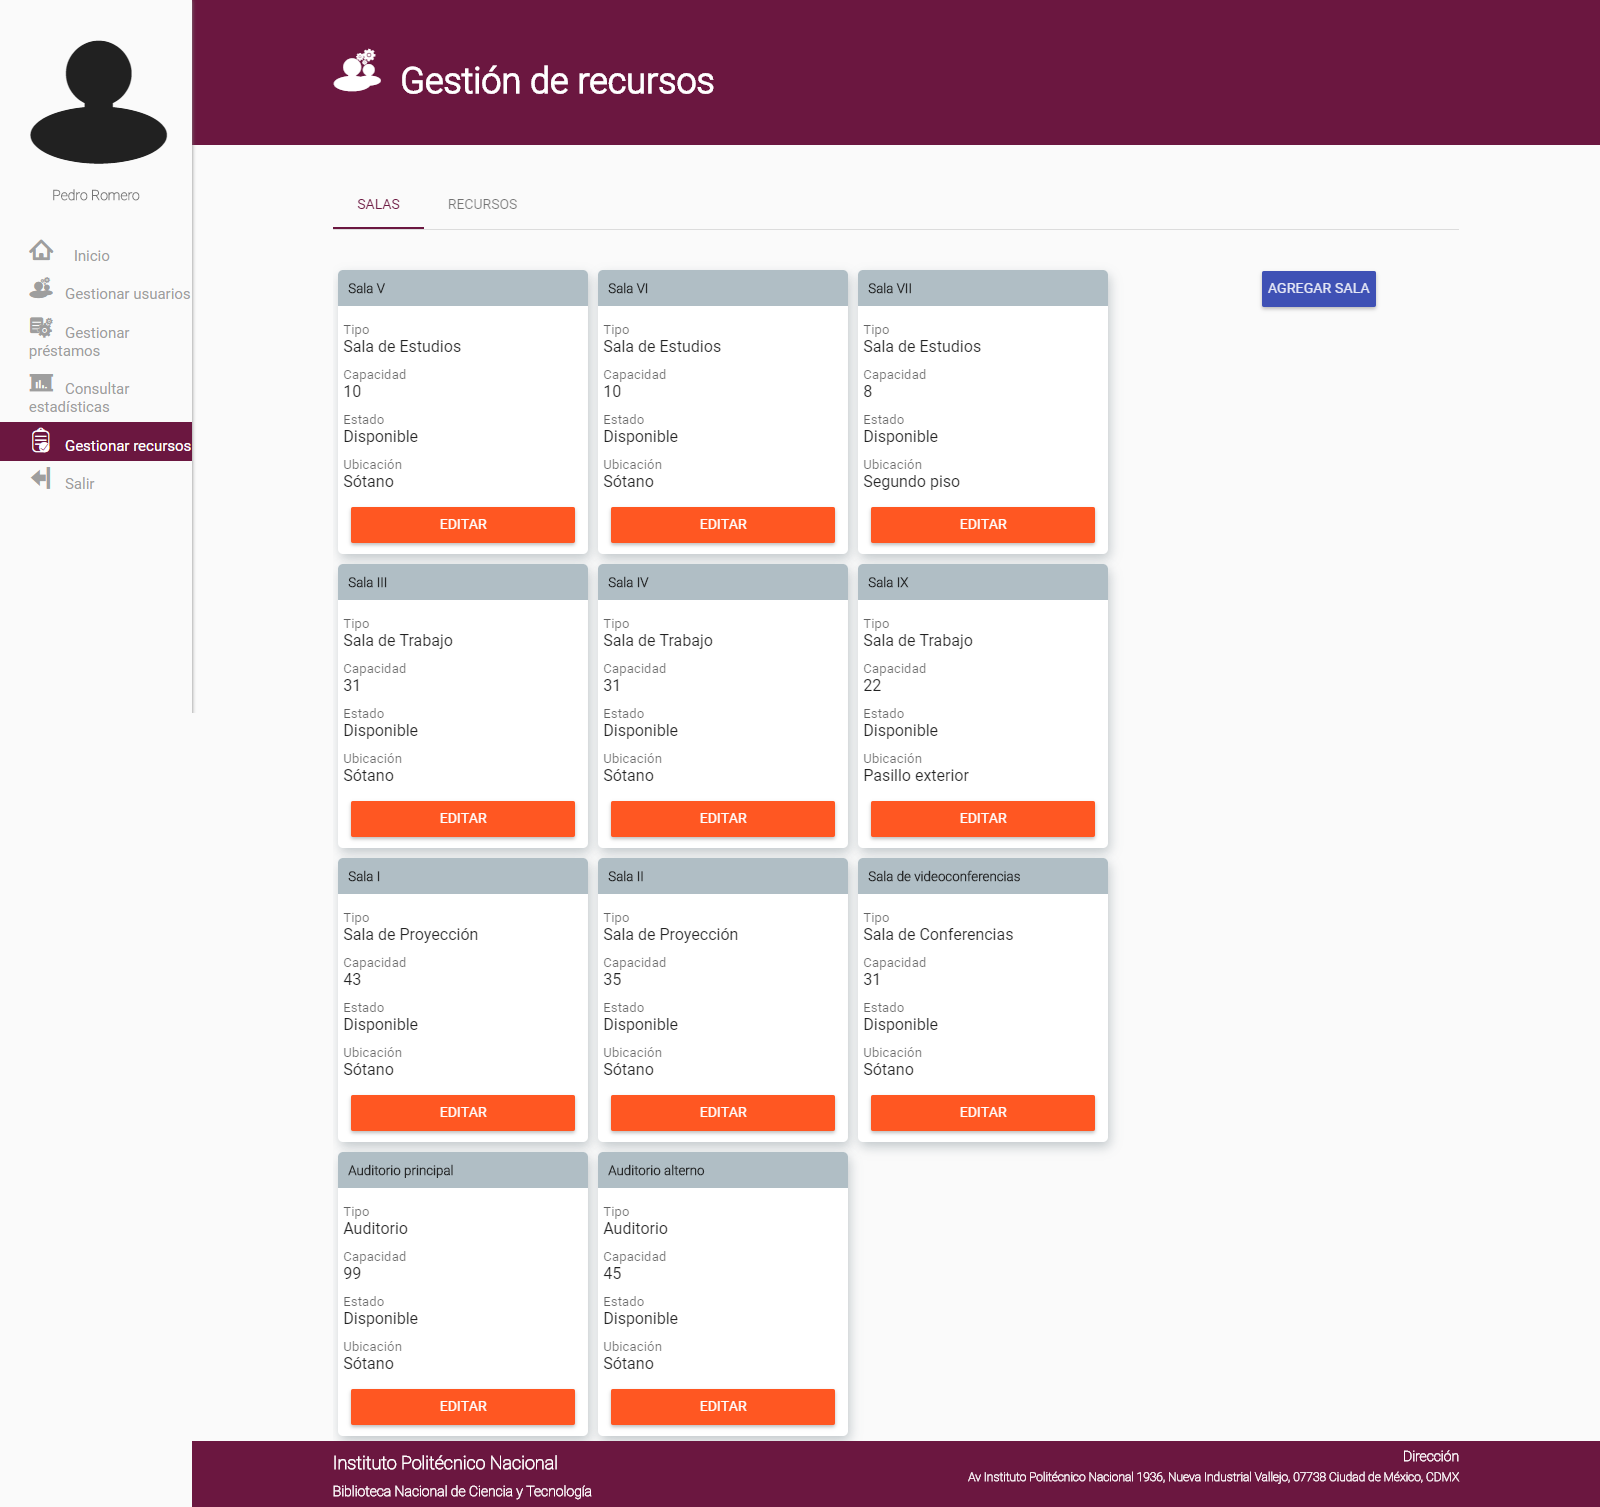
\includegraphics[scale=0.3]{images/Interfaz/IUGS21_GestionarRecursos.png}
				\end{center}
					
			\caption{IUGS-21 Gestionar recursos Sala}
			\end{figure}				
		
		\item Para agregar un recurso presione el botón \textbf{Recurso} \par
		
			\begin{figure}[hbtp]	
				\centering
					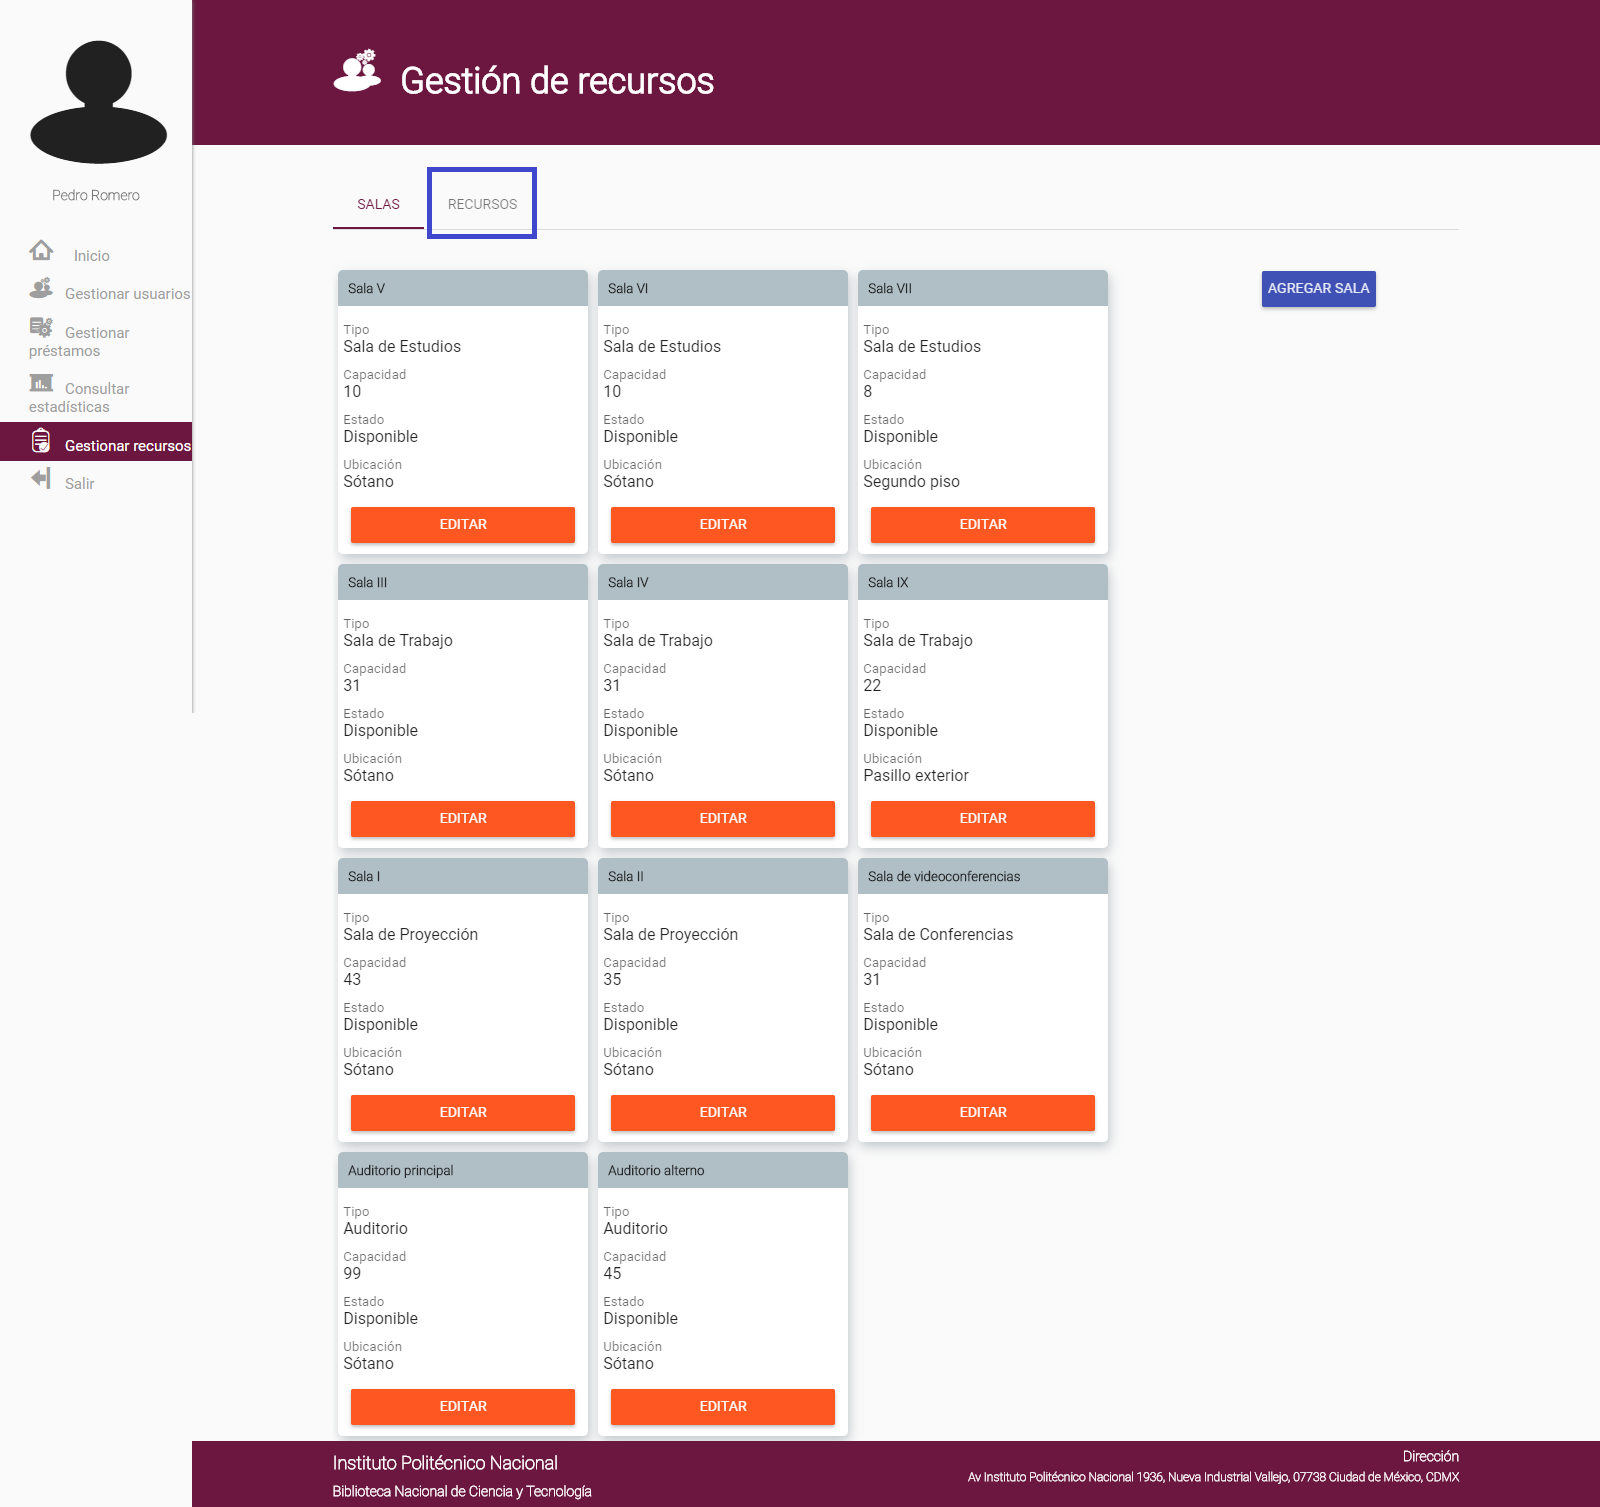
\includegraphics[scale=0.3]{images/Interfaz/IUGS21_GestionarRecursosR.png}
			\caption{IUGS-21 Gestionar recursos}
			\end{figure}
			
			
	\end{enumerate}

	